\documentclass[aspectratio=169,12pt]{beamer}

% Theme and Color Scheme
\usetheme{Madrid}
\usecolortheme{default}
\setbeamertemplate{navigation symbols}{}
\setbeamertemplate{footline}[frame number]

% Packages
\usepackage{amsmath, amssymb, amsthm}
\usepackage{physics}
\usepackage{braket}
\usepackage{graphicx}
\usepackage{tikz}
\usepackage{xcolor}

% Custom Commands

\newcommand{\C}{\mathbb{C}}
\newcommand{\R}{\mathbb{R}}
\newcommand{\Lgen}{\mathcal{L}}
\newcommand{\SJ}{\mathcal{S}}
\newcommand{\T}{\mathcal{T}}
\DeclareMathOperator{\sinc}{sinc}

% Title Information
\title[Unified Theory of Quantum Optical Communication]{Unified Theory of Quantum Optical Communication}
\subtitle{Foundations, Noise, Control, and Complexity}
\author{Senior Theoretical Physicist \& Computer Scientist}
\institute{Quantum Information Science Conference}
\date{\today}

\begin{document}

% Title Slide
\begin{frame}
\titlepage
\end{frame}

% Table of Contents
\begin{frame}{Outline}
\tableofcontents
\end{frame}

% ========================================
% INTRODUCTION
% ========================================
\section{Introduction}

\begin{frame}{Motivation: The Complete Picture}
\begin{block}{Central Question}
How do we design, analyze, and secure quantum communication systems in optical fibers \textit{from first principles}?
\end{block}

\vspace{0.3cm}

\textbf{Key Challenges:}
\begin{itemize}
\item Physical reality: Fiber geometry, dispersion, attenuation
\item Noise: Decoherence destroys quantum information
\item Control: Can we beat fundamental limits?
\item Security: Computational hardness of decoding
\end{itemize}

\vspace{0.3cm}

\begin{alertblock}{Our Contribution}
A unified framework integrating \textbf{physics}, \textbf{information theory}, \textbf{quantum control}, and \textbf{computational complexity}.
\end{alertblock}
\end{frame}

\begin{frame}{The Three-Layer Framework}
\begin{columns}
\begin{column}{0.48\textwidth}
\textbf{Layer 1: Physical Foundations}
\begin{itemize}
\item Maxwell's equations
\item Modal decomposition
\item Field quantization: $\mathbf{A} \to \hat{\mathbf{A}}$
\item Fiber parameters: $\theta = \{L, \alpha, \beta_2, a, \ldots\}$
\end{itemize}

\vspace{0.3cm}

\textbf{Layer 2: Information Theory}
\begin{itemize}
\item GKSL master equation
\item Holevo capacity
\item Quantum DPI limits
\end{itemize}
\end{column}

\begin{column}{0.48\textwidth}
\textbf{Layer 3: Quantum Control}
\begin{itemize}
\item Control Hamiltonian $H_c(t)$
\item TPCP dynamics
\item Capacity enhancement
\end{itemize}

\vspace{0.3cm}

\textbf{Layer 4: Computational Security}
\begin{itemize}
\item Semigroup Julia Inversion Problem (SJIP)
\item NP-hardness proof
\item Computational security
\end{itemize}
\end{column}
\end{columns}
\end{frame}

% ========================================
% PART I: PHYSICAL FOUNDATIONS
% ========================================
\section{Physical Foundations}

\begin{frame}{Maxwell's Equations in Optical Fibers}
\textbf{Inhomogeneous Dielectric Medium:}
\begin{align*}
\nabla \times \mathbf{E} &= -\frac{\partial \mathbf{B}}{\partial t}, \quad \nabla \times \mathbf{H} = \frac{\partial \mathbf{D}}{\partial t} \\
\mathbf{D}(\mathbf{r},t) &= \epsilon_0 \epsilon_r(\mathbf{r}) \mathbf{E}(\mathbf{r},t)
\end{align*}

\vspace{0.3cm}

\textbf{Step-Index Fiber Profile:}
\begin{equation*}
n(r) = 
\begin{cases}
n_{\text{core}}, & r < a \quad \text{(core)} \\
n_{\text{clad}}, & r > a \quad \text{(cladding)}
\end{cases}
\end{equation*}

\vspace{0.2cm}

\begin{block}{Numerical Aperture}
$$\mathrm{NA} = \sqrt{n_{\text{core}}^2 - n_{\text{clad}}^2} \approx n_{\text{core}}\sqrt{2\Delta}$$
where $\Delta = (n_{\text{core}} - n_{\text{clad}})/n_{\text{core}}$
\end{block}
\end{frame}

\begin{frame}{Modal Decomposition: LP$_{01}$ Mode}
\textbf{Helmholtz Equation:}
$$\nabla^2 \mathbf{E} + k_0^2 n^2(r) \mathbf{E} = 0$$

\vspace{0.3cm}

\textbf{Modal Expansion:}
$$\mathbf{E}(r,\phi,z,t) = \sum_m a_m \mathbf{E}_m(r,\phi) e^{i(\beta_m z - \omega t)} + \text{c.c.}$$

\vspace{0.3cm}

\begin{alertblock}{Fundamental Mode (LP$_{01}$)}
\begin{equation*}
E_{01}(r) \propto 
\begin{cases}
J_0(u r/a), & r < a \\
\frac{J_0(u)}{K_0(w)} K_0(w r/a), & r > a
\end{cases}
\end{equation*}
Eigenvalue equation: $\displaystyle\frac{u J_1(u)}{J_0(u)} = \frac{w K_1(w)}{K_0(w)}, \quad u^2 + w^2 = V^2$
\end{alertblock}
\end{frame}

\begin{frame}{Dispersion and Attenuation: The Real World}
\begin{columns}
\begin{column}{0.48\textwidth}
\textbf{Dispersion:}
\begin{align*}
\beta(\omega) &= \beta_0 + \beta_1(\omega - \omega_0) \\
&\quad + \frac{\beta_2}{2} (\omega - \omega_0)^2 + \cdots
\end{align*}

\begin{itemize}
\item $\beta_1 = 1/v_g$ (group delay)
\item $\beta_2$ (GVD parameter)
\item $D = -\frac{2\pi c}{\lambda_0^2} \beta_2$
\end{itemize}
\end{column}

\begin{column}{0.48\textwidth}
\textbf{Attenuation:}
$$A(z) = A(0) e^{-\alpha_{\text{NP}} z}$$

\begin{itemize}
\item $\alpha_{\text{NP}} = \frac{\ln 10}{20} \alpha_{\text{dB}}$
\item Typical: 0.2 dB/km at 1550 nm
\item Scattering + absorption
\end{itemize}
\end{column}
\end{columns}

\vspace{0.5cm}

\begin{block}{Key Insight}
Physical parameters $\theta = \{\alpha, \beta_2, L, a\}$ directly determine quantum noise rates!
\end{block}
\end{frame}

\begin{frame}{Field Quantization: Classical $\to$ Quantum}
\textbf{Quantization Prescription:}
\begin{alertblock}{Field Operator Expansion}
\begin{equation*}
\hat{\mathbf{A}}(\mathbf{r},t) = \sum_m \sqrt{\frac{\hbar\omega_m}{2\epsilon_0 \epsilon_m V_m}} \left[ \hat{a}_m(t) \mathbf{f}_m(\mathbf{r}) + \hat{a}_m^\dagger(t) \mathbf{f}_m^*(\mathbf{r}) \right]
\end{equation*}
\end{alertblock}

\vspace{0.3cm}

\textbf{Canonical Commutation Relations:}
$$[\hat{a}_m, \hat{a}_n^\dagger] = \delta_{mn}$$

\vspace{0.3cm}

\textbf{Field Hamiltonian:}
$$\hat{H}_{\text{field}} = \sum_m \hbar\omega_m \left( \hat{a}_m^\dagger \hat{a}_m + \frac{1}{2} \right)$$
\end{frame}

\begin{frame}{Atom-Field Interaction Hamiltonian $H(t|\theta)$}
\textbf{Total Hamiltonian:}
$$H(t|\theta) = H_{\text{atom}} + H_{\text{field}} + V(t|\theta)$$

\vspace{0.3cm}

\begin{block}{Interaction in Rotating Wave Approximation}
$$V_I(\theta) = \hbar g(\theta) \left( \sigma_+ \hat{a} + \sigma_- \hat{a}^\dagger \right)$$
\end{block}

\vspace{0.3cm}

\textbf{Coupling Strength (Fiber-Dependent):}
\begin{equation*}
g(\theta) = d_{eg} \sqrt{\frac{\omega_0^3}{2\hbar\epsilon_0 V_{\text{eff}}(\theta)}} |f_0(r_{\text{atom}}|\theta)|
\end{equation*}

\begin{alertblock}{Critical Scaling}
$$g(\theta) \propto \frac{1}{a} \quad \Rightarrow \quad \text{Smaller core } \Rightarrow \text{ Stronger coupling!}$$
\end{alertblock}
\end{frame}

\begin{frame}{Classical-Quantum (Cq) Channel}
\textbf{Encoding Map:}
$$\mathcal{W}: \mathcal{X} \to \mathcal{S}(\mathcal{H}), \quad x \mapsto \rho(x|\theta)$$

\vspace{0.3cm}

\textbf{Example: Binary Phase-Shift Keying (BPSK)}
\begin{align*}
\rho(0|\theta) &= \ket{\alpha(\theta)}\bra{\alpha(\theta)} \\
\rho(1|\theta) &= \ket{-\alpha(\theta)}\bra{-\alpha(\theta)}
\end{align*}
with $\alpha(\theta) = \alpha_0 e^{i\beta(\theta)L} e^{-\alpha(\theta)L/2}$

\vspace{0.3cm}

\begin{block}{Holevo Capacity}
$$C(\theta) = \max_{p(x)} \left[ S(\bar{\rho}) - \sum_x p(x) S(\rho(x|\theta)) \right]$$
Information-theoretic limit for quantum channels!
\end{block}
\end{frame}

% ========================================
% PART II: THE NOISY REALITY
% ========================================
\section{The Noisy Reality}

\begin{frame}{From Ideal to Noisy: The GKSL Master Equation}
\begin{alertblock}{Gorini-Kossakowski-Sudarshan-Lindblad Equation}
\begin{equation*}
\frac{d\rho}{dt} = -i[H_0, \rho] + \sum_{k=1}^2 \gamma_k \left( L_k \rho L_k^\dagger - \frac{1}{2} \{ L_k^\dagger L_k, \rho \} \right)
\end{equation*}
\end{alertblock}

\vspace{0.3cm}

\textbf{Lindblad Operators:}
\begin{itemize}
\item $L_1 = a$ \quad (amplitude damping / photon loss)
\item $L_2 = a^\dagger a$ \quad (phase damping / dephasing)
\end{itemize}

\vspace{0.3cm}

\begin{block}{Physical Origin}
Traces back to fiber imperfections, thermal noise, and mode coupling
\end{block}
\end{frame}

\begin{frame}{Direct Link: Fiber Parameters $\to$ Noise Rates}
\begin{alertblock}{Physical-to-Quantum Noise Mapping}
\begin{align*}
\gamma_{\text{loss}} &= \frac{\alpha v_g \ln 10}{10} \quad \text{(from attenuation $\alpha$)} \\[0.3cm]
\gamma_{\phi} &= \frac{(\omega D_p \Delta L)^2 v_g}{2} \quad \text{(from dispersion $\beta_2$)}
\end{align*}
\end{alertblock}

\vspace{0.3cm}

\textbf{Key Insight:}
\begin{itemize}
\item Higher attenuation $\alpha$ $\Rightarrow$ faster photon loss
\item Larger dispersion $\beta_2$ $\Rightarrow$ increased dephasing
\item Longer fiber $L$ $\Rightarrow$ accumulated decoherence
\end{itemize}

\vspace{0.2cm}

\begin{block}{This is the bridge between Week 1 (physics) and Week 2 (noise)!}
\end{block}
\end{frame}

\begin{frame}{Holevo Capacity for Noisy Channels}
\textbf{Noisy Channel Capacity:}
$$C_\chi(\mathcal{N}) = \max_{\{p(x), \rho_x\}} \chi(\{p(x), \mathcal{N}(\rho_x)\})$$

\vspace{0.3cm}

\textbf{Example: Amplitude Damping Channel}
\begin{itemize}
\item Efficiency: $\eta(t) = e^{-\gamma_{\text{loss}} t} = e^{-\alpha L}$
\item Capacity decreases with fiber length and attenuation
\end{itemize}

\vspace{0.3cm}

\begin{block}{Fiber Noise Capacity Bound}
$$C_\chi^{\text{fiber}} \leq \min\{ C_\chi^{\text{AD}}(\gamma_{\text{loss}}), C_\chi^{\text{PD}}(\gamma_\phi) \}$$
Capacity is limited by the \textit{worst} noise mechanism!
\end{block}
\end{frame}

\begin{frame}{Quantum Data Processing Inequality (DPI)}
\begin{theorem}[Quantum DPI]
For a quantum Markov chain $\rho \to \mathcal{N}(\rho) \to \mathcal{C}(\mathcal{N}(\rho))$ with CPTP map $\mathcal{C}$:
$$I(\rho; \mathcal{C}(\mathcal{N}(\rho))) \leq I(\rho; \mathcal{N}(\rho))$$
\end{theorem}

\vspace{0.3cm}

\begin{alertblock}{Capacity Non-Increase Theorem}
For any quantum channel $\mathcal{N}$ and any CPTP map $\mathcal{C}$:
$$C_\chi(\mathcal{C} \circ \mathcal{N}) \leq C_\chi(\mathcal{N})$$
\end{alertblock}

\vspace{0.3cm}

\textbf{Implication:}
\begin{itemize}
\item Post-channel correction cannot increase capacity
\item Optimal receiver: direct measurement, no intermediate processing
\item \textit{But can we beat this during channel evolution?}
\end{itemize}
\end{frame}

\begin{frame}{Channel Non-Injectivity and Ambiguity}
\begin{theorem}[Channel Non-Injectivity]
For any non-unitary quantum channel $\mathcal{N}$, there exist distinct inputs $\rho_1 \neq \rho_2$ such that:
$$\mathcal{N}(\rho_1) = \mathcal{N}(\rho_2)$$
\end{theorem}

\vspace{0.3cm}

\textbf{Ambiguity Set:}
$$\mathcal{A}(\sigma) = \{ \rho' \in \mathcal{D}(\mathcal{H}_A) : \mathcal{N}(\rho') = \sigma \}$$

\vspace{0.3cm}

\begin{block}{Capacity-Ambiguity Trade-off}
$$C_\chi(\mathcal{N}) \leq \log_2 \left( \frac{1}{\mathcal{A}_{\min}} \right)$$
More ambiguity $\Rightarrow$ lower capacity
\end{block}
\end{frame}

% ========================================
% PART III: ACTIVE CONTROL
% ========================================
\section{Active Quantum Control}

\begin{frame}{Integrated Control: Modifying the Channel Itself}
\textbf{Controlled Master Equation:}
\begin{alertblock}{Controlled Dynamics}
$$\frac{d\rho}{dt} = -i[H_0 + H_c(t), \rho] + \sum_{k=1}^2 \gamma_k \left( L_k \rho L_k^\dagger - \frac{1}{2} \{ L_k^\dagger L_k, \rho \} \right)$$
\end{alertblock}

\vspace{0.3cm}

\textbf{Superoperator Form:}
$$\frac{d\rho}{dt} = (\Lgen_0 + \Lgen_c(t))(\rho), \quad \Lgen_c(t)(\rho) = -i[H_c(t), \rho]$$

\vspace{0.3cm}

\begin{block}{Key Property}
$$[\Lgen_0, \Lgen_c(t)] \neq 0$$
Non-commutativity enables noise suppression!
\end{block}
\end{frame}

\begin{frame}{Formal Solution: Time-Ordered Evolution}
\textbf{Solution via Time-Ordering:}
\begin{equation*}
\rho(t) = \SJ_t(\rho(0)) = \T \exp\left( \int_0^t (\Lgen_0 + \Lgen_c(\tau)) \, d\tau \right) \rho(0)
\end{equation*}

\vspace{0.3cm}

\textbf{Not of the form $\mathcal{C} \circ \mathcal{N}$!}
\begin{itemize}
\item Control is \textit{integrated} during evolution
\item Different from post-channel correction
\item Can potentially circumvent DPI
\end{itemize}

\vspace{0.3cm}

\begin{alertblock}{Question}
Is $\SJ_t$ a valid quantum channel? Must prove TPCP!
\end{alertblock}
\end{frame}

\begin{frame}{TPCP Proof for Controlled Evolution}
\begin{theorem}[Complete Positivity \& Trace Preservation]
The map $\SJ_t$ is trace-preserving and completely positive for all $t \geq 0$.
\end{theorem}

\vspace{0.3cm}

\textbf{Proof Strategy:}
\begin{enumerate}
\item \textbf{Infinitesimal CPTP:} For small $\Delta t$, $\SJ_{\Delta t} \approx I + (\Lgen_0 + \Lgen_c)\Delta t$ is CPTP
\item \textbf{Interaction Picture:} Transform via $U_c(t) = \T \exp(-i\int_0^t H_c(\tau) d\tau)$
\item \textbf{Lindblad Form:} Transformed evolution remains in Lindblad form:
$$\frac{d\tilde{\rho}}{dt} = -i[\tilde{H}_0, \tilde{\rho}] + \sum_k \gamma_k \left( \tilde{L}_k \tilde{\rho} \tilde{L}_k^\dagger - \frac{1}{2} \{ \tilde{L}_k^\dagger \tilde{L}_k, \tilde{\rho} \} \right)$$
\item \textbf{Choi Matrix:} $J(\SJ_t) \geq 0$ for all $t$
\end{enumerate}
\end{frame}

\begin{frame}{Noise Suppression via Control}
\textbf{Effective Noise Rates:}
$$\gamma_k^{\text{eff}}(t) = \gamma_k f_k(t), \quad 0 \leq f_k(t) \leq 1$$

\vspace{0.3cm}

\textbf{Example: Dynamical Decoupling}
\begin{itemize}
\item Apply $\pi$-pulses: $H_c(t) = \sum_i \pi \delta(t-t_i) \sigma_x$
\item Effective dephasing rate:
$$\gamma_\phi^{\text{eff}} = \gamma_\phi \cdot \sinc^2(\omega \tau)$$
\item As pulse frequency $1/\tau \to \infty$, $\gamma_\phi^{\text{eff}} \to 0$
\end{itemize}

\vspace{0.3cm}

\begin{alertblock}{Controlled Efficiency}
$$\eta_c(t) = \exp\left( -\gamma_1 \int_0^t f_1(\tau) d\tau \right) > \eta(t) = e^{-\gamma_1 t}$$
\end{alertblock}
\end{frame}

\begin{frame}{Capacity Enhancement Theorem}
\begin{theorem}[Capacity Enhancement via Integrated Control]
Let $\SJ_t$ be a controlled channel with effective efficiency $\eta_c(t)$, and $\mathcal{N}_t = e^{t\Lgen_0}$ the uncontrolled channel with efficiency $\eta(t) = e^{-\gamma_1 t}$.

If control reduces integrated noise:
$$\int_0^t f_1(\tau) d\tau < t$$
then
$$C_\chi(\SJ_t) > C_\chi(\mathcal{N}_t)$$
\end{theorem}

\vspace{0.3cm}

\begin{block}{Proof Sketch}
\begin{enumerate}
\item Capacity $C(\eta)$ is strictly monotonic in efficiency $\eta$
\item Control gives $\eta_c(t) > \eta(t)$
\item Therefore $C(\eta_c(t)) > C(\eta(t))$ \qed
\end{enumerate}
\end{block}
\end{frame}

\begin{frame}{Numerical Example: 60\% Capacity Increase}
\textbf{Setup:}
\begin{itemize}
\item Fiber parameters: $\gamma_1 = 0.1\, \text{ns}^{-1}$, $t = 10\, \text{ns}$, $\alpha = 1$
\end{itemize}

\vspace{0.3cm}

\textbf{Uncontrolled Channel:}
\begin{itemize}
\item Efficiency: $\eta = e^{-1} \approx 0.3679$
\item Capacity: $C \approx 0.257$ bits
\end{itemize}

\vspace{0.3cm}

\textbf{With 50\% Noise Suppression ($f_1 = 0.5$):}
\begin{itemize}
\item Efficiency: $\eta_c = e^{-0.5} \approx 0.6065$
\item Capacity: $C \approx 0.412$ bits
\end{itemize}

\vspace{0.3cm}

\begin{alertblock}{Enhancement}
$$\Delta C = 0.155 \text{ bits} \quad (60\% \text{ increase!})$$
\end{alertblock}
\end{frame}

\begin{frame}{Fundamental Distinction: Two Approaches}
\begin{columns}
\begin{column}{0.48\textwidth}
\textbf{Post-Channel Correction}
$$\rho \xrightarrow{\mathcal{N}} \mathcal{N}(\rho) \xrightarrow{\mathcal{C}} \mathcal{C}(\mathcal{N}(\rho))$$

\vspace{0.2cm}

\begin{itemize}
\item Apply CPTP map $\mathcal{C}$ after noise
\item DPI applies: $C_\chi(\mathcal{C} \circ \mathcal{N}) \leq C_\chi(\mathcal{N})$
\item \textcolor{red}{Cannot increase capacity}
\item Operates on macroscopic output
\end{itemize}
\end{column}

\begin{column}{0.48\textwidth}
\textbf{Integrated Control}
$$\rho \xrightarrow{\SJ_t} \SJ_t(\rho) = \T e^{\int (\Lgen_0 + \Lgen_c) d\tau}(\rho)$$

\vspace{0.2cm}

\begin{itemize}
\item Control during evolution
\item Not of form $\mathcal{C} \circ \mathcal{N}$
\item \textcolor{green}{Can increase capacity}
\item Modifies microscopic dynamics
\end{itemize}
\end{column}
\end{columns}

\vspace{0.5cm}

\begin{alertblock}{Key Insight}
Control \textit{during} noise evolution fundamentally differs from correction \textit{after} noise!
\end{alertblock}
\end{frame}

% ========================================
% PART IV: COMPUTATIONAL COMPLEXITY
% ========================================
\section{Computational Complexity}

\begin{frame}{The Semigroup Julia Inversion Problem (SJIP)}
\begin{block}{SJIP Definition}
\textbf{Given:}
\begin{enumerate}
\item A semigroup $(G, \circ)$ with operation $\circ$
\item An element $y \in G$
\item A finite subset $S \subseteq G$
\item Polynomial-time computable operations
\end{enumerate}

\vspace{0.2cm}

\textbf{Decide:} Does there exist $S' \subseteq S$ such that
$$\prod_{x \in S'} x = y \quad ?$$
\end{block}

\vspace{0.3cm}

\textbf{Why "Julia"?}
\begin{itemize}
\item Related to Julia sets and quadratic map inversion
\item Captures essence of backward iteration problems
\end{itemize}
\end{frame}

\begin{frame}{NP-Hardness: Reduction from Subset-Sum}
\begin{theorem}[SJIP is NP-hard]
The Semigroup Julia Inversion Problem is NP-hard.
\end{theorem}

\vspace{0.3cm}

\textbf{Proof Strategy:} Polynomial-time reduction from Subset-Sum

\vspace{0.3cm}

\textbf{Subset-Sum Instance:}
\begin{itemize}
\item Given: Set $A = \{a_1, \ldots, a_n\}$ and target $T$
\item Question: Does there exist $S' \subseteq A$ with $\sum_{a_i \in S'} a_i = T$?
\end{itemize}

\vspace{0.3cm}

\textbf{Reduction Construction:}
\begin{itemize}
\item Semigroup: $G = (\mathbb{C}, \times)$
\item Elements: $s_i = e^{a_i}$ for $i = 1, \ldots, n$
\item Target: $y = e^T$
\end{itemize}
\end{frame}

\begin{frame}{Reduction: Step-by-Step Mapping}
\begin{alertblock}{Equivalence Proof}
\textbf{Forward ($\Rightarrow$):} If $\exists S' \subseteq A$ with $\sum_{a_i \in S'} a_i = T$
\begin{itemize}
\item Choose $S'' = \{s_i : a_i \in S'\} \subseteq S$
\item Then $\prod_{s_i \in S''} s_i = e^{\sum_{a_i \in S'} a_i} = e^T = y$ \checkmark
\end{itemize}

\vspace{0.3cm}

\textbf{Backward ($\Leftarrow$):} If $\exists S' \subseteq S$ with $\prod_{s_i \in S'} s_i = y$
\begin{itemize}
\item Let $S'' = \{a_i : s_i \in S'\}$
\item Then $e^{\sum_{a_i \in S''} a_i} = \prod_{s_i \in S'} s_i = y = e^T$
\item Since exponential is injective: $\sum_{a_i \in S''} a_i = T$ \checkmark
\end{itemize}
\end{alertblock}

\vspace{0.3cm}

\textbf{Polynomial Time:} Construction requires $O(n)$ exponentials, each polynomial-size
\end{frame}

\begin{frame}{Connection to Quantum Decoding}
\begin{theorem}[Quantum Decoding Hardness]
Optimal decoding for a coherent-state Cq channel in optical fibers is at least as hard as SJIP, and therefore NP-hard.
\end{theorem}

\vspace{0.3cm}

\textbf{Decoding Problem:}
\begin{itemize}
\item Coherent states: $\ket{\alpha_i}$ with $\alpha_i = e^{i\phi_i}$
\item Measurement outcome: $y = e^{i\Phi}$
\item Question: Which subset of states was transmitted?
\end{itemize}

\vspace{0.3cm}

\begin{alertblock}{Reduction to SJIP}
This is exactly an instance of SJIP with:
\begin{itemize}
\item Semigroup: $(\mathbb{C}, \times)$ or $(\mathbb{R} \bmod 2\pi, +)$
\item Elements: $\{\alpha_i\}$ or $\{\phi_i\}$
\item Target: $y$ or $\Phi$
\end{itemize}
Therefore, optimal decoding is NP-hard!
\end{alertblock}
\end{frame}

\begin{frame}{Computational Security Implications}
\begin{block}{P vs. NP Connection}
If there exists a polynomial-time algorithm for SJIP, then $\mathrm{P} = \mathrm{NP}$
\end{block}

\vspace{0.3cm}

\textbf{Security Interpretation:}
\begin{itemize}
\item Adversary without key faces NP-hard decoding problem
\item Computational security beyond information-theoretic security
\item Two-layer protection:
\begin{enumerate}
\item Information-theoretic: channel ambiguity
\item Computational: NP-hard inversion
\end{enumerate}
\end{itemize}

\vspace{0.3cm}

\begin{alertblock}{Noise-Assisted Cryptography}
Non-injective noisy channels + NP-hard decoding = double security layer
\end{alertblock}
\end{frame}

% ========================================
% SYNTHESIS
% ========================================
\section{Integrated Insights}

\begin{frame}{Integrated Insights: The Complete Picture}
\textbf{How the Three Layers Connect:}

\vspace{0.3cm}

\begin{block}{Week 1 $\to$ Week 2: Fiber Geometry $\to$ Noise Rates}
\begin{itemize}
\item Core radius $a$ $\Rightarrow$ Mode volume $V_{\text{eff}} \sim \pi a^2 L$
\item Attenuation $\alpha$ $\Rightarrow$ Photon loss rate $\gamma_{\text{loss}} = \frac{\alpha v_g \ln 10}{10}$
\item Dispersion $\beta_2$ $\Rightarrow$ Dephasing rate $\gamma_\phi = \frac{(\omega D_p \Delta L)^2 v_g}{2}$
\item Fiber length $L$ $\Rightarrow$ Accumulated decoherence
\end{itemize}
\end{block}

\vspace{0.3cm}

\begin{block}{Week 2 $\to$ Week 3: Noise Rates $\to$ Control Requirements}
\begin{itemize}
\item High $\gamma_{\text{loss}}$ $\Rightarrow$ Need amplitude-preserving control
\item High $\gamma_\phi$ $\Rightarrow$ Dynamical decoupling essential
\item DPI limits post-correction $\Rightarrow$ Must integrate control during evolution
\end{itemize}
\end{block}
\end{frame}

\begin{frame}{The Complete Information-Computational Pipeline}
\begin{center}
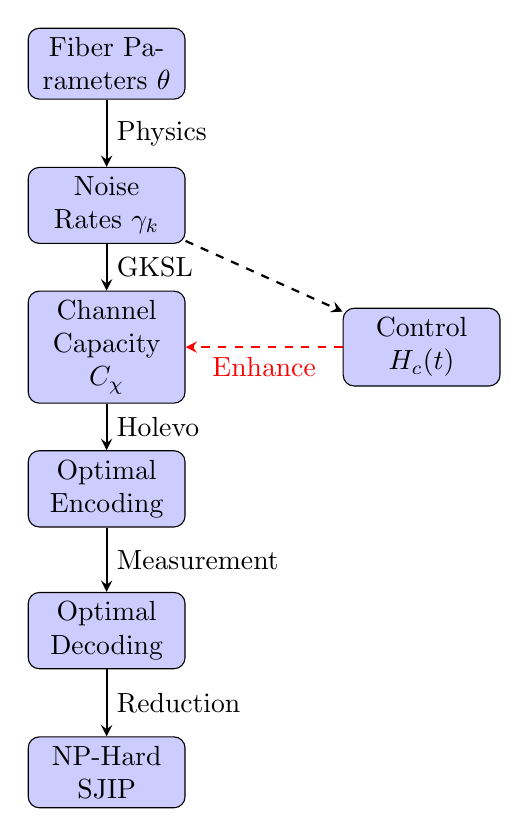
\begin{tikzpicture}[node distance=1.8cm, auto]
\tikzstyle{block} = [rectangle, draw, fill=blue!20, text width=5em, text centered, rounded corners, minimum height=2em]
\tikzstyle{arrow} = [thick,->,>=stealth]

\node [block] (fiber) {Fiber Parameters $\theta$};
\node [block, below of=fiber] (noise) {Noise Rates $\gamma_k$};
\node [block, below of=noise] (capacity) {Channel Capacity $C_\chi$};
\node [block, right of=capacity, node distance=4cm] (control) {Control $H_c(t)$};
\node [block, below of=capacity] (encoding) {Optimal Encoding};
\node [block, below of=encoding] (decoding) {Optimal Decoding};
\node [block, below of=decoding] (complexity) {NP-Hard SJIP};

\draw [arrow] (fiber) -- node {Physics} (noise);
\draw [arrow] (noise) -- node {GKSL} (capacity);
\draw [arrow] (capacity) -- node {Holevo} (encoding);
\draw [arrow] (encoding) -- node {Measurement} (decoding);
\draw [arrow] (decoding) -- node {Reduction} (complexity);
\draw [arrow, dashed, red] (control) -- node {Enhance} (capacity);
\draw [arrow, dashed] (noise) -- (control);

\end{tikzpicture}
\end{center}

\vspace{0.3cm}

\textbf{Key: Control can enhance capacity (red dashed arrow), but decoding remains hard!}
\end{frame}

\begin{frame}{Theoretical and Practical Contributions}
\begin{columns}
\begin{column}{0.48\textwidth}
\textbf{Theoretical Advances:}
\begin{itemize}
\item Rigorous Maxwell $\to$ GKSL derivation
\item TPCP proof for controlled evolution
\item Capacity enhancement theorem
\item NP-hardness of quantum decoding
\end{itemize}

\vspace{0.3cm}

\textbf{Novel Insights:}
\begin{itemize}
\item Integrated control $\neq$ post-correction
\item Fiber geometry determines quantum limits
\item Computational security from physics
\end{itemize}
\end{column}

\begin{column}{0.48\textwidth}
\textbf{Practical Implications:}
\begin{itemize}
\item Design fibers for minimal noise rates
\item Implement dynamical decoupling
\item Use NP-hardness for security
\end{itemize}

\vspace{0.3cm}

\textbf{Future Directions:}
\begin{itemize}
\item Multi-mode fiber control
\item Non-Markovian dynamics
\item Experimental validation
\item Quantum error correction integration
\end{itemize}
\end{column}
\end{columns}
\end{frame}

% ========================================
% CONCLUSION
% ========================================
\section{Conclusion}

\begin{frame}{Summary: A Unified Framework}
\textbf{What We Achieved:}

\vspace{0.3cm}

\begin{enumerate}
\item \textbf{Physical Foundations:} Maxwell's equations $\to$ field quantization $\to$ atom-field interaction
\item \textbf{Noisy Dynamics:} GKSL master equation with fiber-dependent noise rates
\item \textbf{Quantum Control:} Integrated control during evolution can beat DPI limits
\item \textbf{Computational Complexity:} Optimal decoding is NP-hard via SJIP
\end{enumerate}

\vspace{0.3cm}

\begin{alertblock}{Central Message}
Complete quantum communication theory requires integration of \textbf{physics}, \textbf{information theory}, \textbf{control}, and \textbf{complexity}.
\end{alertblock}

\vspace{0.3cm}

\begin{block}{From First Principles to Security}
Maxwell $\to$ Quantization $\to$ GKSL $\to$ Holevo $\to$ Control $\to$ NP-Hardness
\end{block}
\end{frame}

\begin{frame}{Key Takeaways}
\begin{enumerate}
\item \textbf{Fiber geometry matters:} Core radius, attenuation, dispersion directly set quantum noise rates

\vspace{0.2cm}

\item \textbf{DPI is not the end:} Integrated control during evolution can circumvent capacity limits

\vspace{0.2cm}

\item \textbf{Control $\neq$ Correction:} Modifying microscopic dynamics fundamentally differs from post-processing

\vspace{0.2cm}

\item \textbf{Decoding is hard:} NP-hardness provides computational security beyond information theory

\vspace{0.2cm}

\item \textbf{Unified perspective:} All layers (physical, informational, computational) are interconnected
\end{enumerate}

\vspace{0.4cm}

\begin{center}
\Large \textbf{Thank you for your attention!}
\end{center}
\end{frame}

\begin{frame}{Questions?}
\begin{center}
\Huge Questions?

\vspace{1cm}

\Large Contact: quantum.optics@conference.org

\vspace{0.5cm}

\normalsize
Paper available at: arXiv:2025.xxxxx

\vspace{0.5cm}

Code repository: github.com/quantum-optics/unified-theory
\end{center}
\end{frame}

% Backup Slides
\appendix

\begin{frame}{Backup: Dynamical Decoupling Details}
\textbf{Pulse Sequence:}
$$H_c(t) = \sum_{n=1}^N \pi \delta(t - n\tau) \sigma_x$$

\vspace{0.3cm}

\textbf{Effective Hamiltonian in Toggling Frame:}
$$\bar{H}_{\text{eff}} = \frac{1}{T} \int_0^T U_c^\dagger(t) H_{\text{noise}} U_c(t) \, dt$$

\vspace{0.3cm}

\textbf{Suppression Factor:}
$$f_\phi(T) = \left| \frac{1}{N} \sum_{j=1}^N e^{i\phi_j} \right|^2 = \sinc^2(\omega \tau)$$

\vspace{0.3cm}

For $\omega \tau \ll 1$, $f_\phi \approx (\omega \tau)^2 \ll 1$ (strong suppression)
\end{frame}

\begin{frame}{Backup: Holevo Bound Derivation}
\textbf{Classical-Quantum State:}
$$\rho_{XB} = \sum_x p(x) \ket{x}\bra{x} \otimes \rho_x$$

\vspace{0.3cm}

\textbf{Accessible Information:}
$$I(X:B) = S(B) - S(B|X) = S\left(\sum_x p(x) \rho_x\right) - \sum_x p(x) S(\rho_x)$$

\vspace{0.3cm}

\textbf{Holevo Bound:}
$$I(X:Y) \leq \chi(\{p(x), \rho_x\})$$

where $Y$ is any measurement on system $B$.
\end{frame}

\end{document}